\Chapter{System Design}
\lstset{breaklines=true}

\section{Design Overview}
The GradeBadge application uses a client-server architecture model, and it uses the Model View Controller (MVC) architecture model for both client and server, as shown in Figure~\ref{fig:mvc}.  All communication between client and server is done through AJAX requests submitted through HTTP POST and containing data encoded using JSON. 

\vspace{3em}
\begin{figure}[H]
\begin{center}
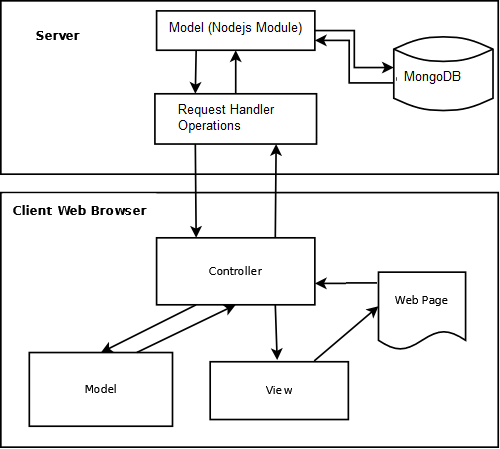
\includegraphics[height=3.1in,width=3.5in]{images/mvc_diagram.png}
\caption{GradeBadge MVC Architecture}
\label{fig:mvc}
\end{center}
\end{figure}   

\section{Model View Controller Architecture}
This application is based on the Model View Controller (MVC) architecture,
which is a software design pattern for separating different components of a software application \cite{MVC}. There are three main components in the MVC architecture as follows.

\begin{itemize}
\item Model: The model includes data in the application and the business rules that apply to it.
\item View: The view includes the UI components in the application. The UI components are responsible for presenting the model and for collecting user input.
\item Controller: The controller is responsible for updating the data in the model and notifying the view about changes in the model.
\end{itemize}

\section{Bandwidth Reduction Strategy}
The following sections describe the three strategies used in this project to reduce consumption of bandwidth.  Bandwidth is one of the major costs to consider when building a scalable application using cloud computing services, so minimizing bandwidth consumption becomes critical.

\subsection{File Compression}
In this application, in order to reduce the bandwidth consumption, files that are transferred from the application server will be compressed in the gzip format if the client browser supports it, which will result in smaller files. The following code shows how browser requests for static resources are tested to see if the browser supports gzip compression.  This code appears in the req{\_}file module.

\begin{lstlisting}
if (file.gzip !== undefined && 
  req.headers['accept-encoding'] !== undefined && 
  req.headers['accept-encoding'].indexOf('gzip') !== -1) 
{
  return app_http.replyCached(res, file.gzip, file.type, file.etag, 'gzip');
} else {
  return app_http.replyCached(res, file.data, file.type, file.etag);
}
\end{lstlisting}

In addition to checking whether the browser supports gzip compression, the above code also checks for any etag value sent by the browser.  The etag functions as a version identifier, which the browser sends to the server with the request message to see whether the file is different from what is in the browser cache and what the server would return.  If the etag indicates that the file is current, the server doesn't need to return the file; it simply returns a code indicating that the browser's cached version of the file is current. The following shows how this is done in code.
 
\begin{lstlisting}
  if (req.headers['if-none-match'] === file.etag) {
    return app_http.replyNotModified(res);
  }
\end{lstlisting}

\subsection{Content Distribution Network Resources}
In this application, we rely on content distribution networks (CDNs) to deliver some static resources to browsers without consuming bandwidth to the application server.  For example, the application relies on the Bootstrap UI framework.  The files for this framework are available through a CDN provided for free to application developers.  The following code shows how GradeBadge loads the CSS component of the Bootstrap system.
\begin{lstlisting}
<link href="//netdna.bootstrapcdn.com/twitter-bootstrap/
    2.2.2/css/bootstrap.css" rel="stylesheet">
\end{lstlisting}

\subsection{Caching}
In this application, we implemented a caching strategy in which every request is checked to see whether a needed file has been modified or is cached in the client browser. This is done by examining an etag value that identifies a version of the requested file.  If the browser's version of the file is current, then the server replies with a code of 304, which indicates that the file is current.  If the etag does not identify the current version of the file, then the server return the current version of the file. This strategy is implemented to reduce unnecessary consumption of bandwidth.

The following describes the four possible responses from the server when the browser requests a file.  The source code is taken from the app{\_}http modul. 

\begin{itemize}
\item Reply Not Found: This is the response when the requested file is not found; the server returns the code 404, as shown in the following code snippet.

\begin{lstlisting}
res.writeHead(404, {});
\end{lstlisting}

\item Reply Not Modified: This is the response when the requested file is not modified as determined by comparing the browser's etag with the server's etag. The following shows how this is done in the code.  Note that the server takes this opportunity to reset the expiration time of the requested file to one year later. 

\begin{lstlisting}
res.writeHead(304, {
    'Connection'       : 'keep-alive',
    'Proxy-Connection' : 'keep-alive',
    'Cache-Control'    : 'max-age=31536000',
    'Expires'          : new Date(Date.now() + 31536000000)
  });
\end{lstlisting}

\item Reply Not Cached: This is the response when the requested file is not cached in the client browser. The following shows how this is done in the code, where the server responds by returning the requested file.

\begin{lstlisting}
res.writeHead(200, {
    'Content-Type'     : 'text/html',
    'Content-Length'   : buffer.length,
    'Connection'       : 'keep-alive',
    'Proxy-Connection' : 'keep-alive',
    'Pragma'           : 'no-cache',
    'Cache-Control'    : 'no-cache, no-store'
  });
\end{lstlisting}

\item Reply Cached: This is the response when the requested file is cached in the client browser, in which case the server will reset the expiration date of the file to one year later. The following shows how this is done in the code.

\begin{lstlisting}
    res.writeHead(200, {
      'Content-Type'     : contentType,
      'Content-Length'   : buffer.length,
      'Connection'       : 'keep-alive',
      'Proxy-Connection' : 'keep-alive',
      'Pragma'           : 'public',
      'Cache-Control'    : 'max-age=31536000',
      'Vary'             : 'Accept-Encoding',
      'Expires'          : new Date(Date.now() + 31536000000),
      'ETag'             : etag,
      'Content-Encoding' : contentEncoding
    });
\end{lstlisting}

\end{itemize}


\section{Server-side Design}

\subsection{Request Processing}
In Nodejs, components are organized into modules, which can function as namespaces. In this project, all Nodejs modules that start with req{\_} are request handlers that get requested from the router module. All Ajax requests will go through the req{\_}op module, which verifies that the user is logged into Facebook and the application version is current. Every request passing through req{\_}op must contain a Facebook access token and application version identifier. If the user is not logged into Facebook, then req{\_}op returns the JSON document {login:true}. If the application version is not current, then req{\_}op returns the JSON document {ver:true}, as shown Figure~\ref{fig:sequence}

\vspace{3em}
\begin{figure}[H]
\begin{center}
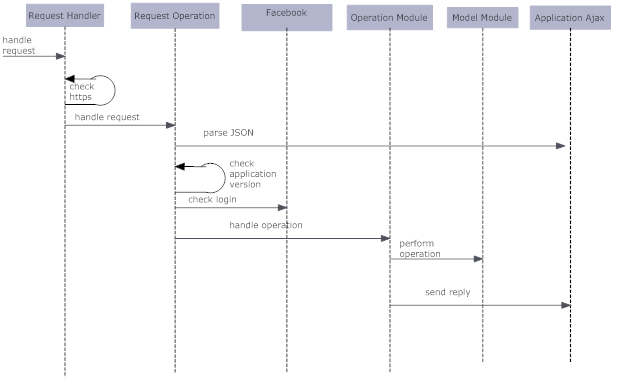
\includegraphics[height=3.1in,width=5.5in]{images/sequence.png}
\caption{Request Processing Sequence Diagram}
\label{fig:sequence}
\end{center}
\end{figure}   

\subsection{Configuration}
The following are the list of configuration files required on the server side.

\begin{itemize}
\item .env: This is the setup file that contains environmental variables. This file only exists in the developer local environment.  The same environmental variables need to be present in the Heroku execution environment, however, they are specified through another mechanism, namely through executing the Heroku config command for both staging and production environments.

The following is an example of the environmental variable values that could be set in the development environment. In this example, FB{\_}APP{\_}ID is the Facebook application ID and FB{\_}SECRET is the Facebook application secret. (For each environment, we are using a different Facebook application instance.)  PORT is the HTTP port number that the server will listen to for connections. APP{\_}VER is the current application version. MONGO{\_}URI is the mongo database connection string. (We use different database instances for each environment.)
\begin{lstlisting}
FB_APP_ID=466760923387961
FB_SECRET=75e7a042473a989a3b876d3ec8749920
PORT=5000
APP_VER=2
MONGO_URI=mongodb://app:gradebadge123@
         ds045757.mongolab.com:45757/gb-d
\end{lstlisting} 

\item .gitignore: This is the setup file that contains matching patterns that tell git which files should be ignored (not placed under version control) when committing to a branch of the local repository. 
\item .slugignore: This is the setup file that contains a list of files or folders that will be ignored when calculating the slug limit in Heroku.
\item package.json: This is the setup file that contains a list of Nodejs dependencies and engine version to use when deploying the application. This file also contains the application name, version and description, as shown in the following. 
\begin{lstlisting}
{
    "name": "gradebadge",
    "version": "0.0.1",
    "description": "Grade Badge System",
    "dependencies": {
        "mongodb": "1.2.13"
    },
    "engines": {
        "node": "0.8.21",
        "npm": "1.2.12"
    }
}
\end{lstlisting} 

\item Procfile: This is the setup file that tells Heroku how to launch the application, as shown in the following.
\begin{lstlisting}
web: node main.js
\end{lstlisting} 

\end{itemize}

\subsection{Nodejs Modules}
Below are the list of files that are used when the server executes.

\begin{itemize}
\item main.js: This is the main module in Nodejs, which contains code that verifies all necessary environmental variables are set correctly. It also invokes initialization functions of other modules to start the application.  After initialization is complete, the main module starts the HTTP request handling loop. 

The following is the part of the code in the main module where it initializes the model, router and fb modules and runs them asynchronously. 
\begin{lstlisting}
var n = 3;
function done() {
  if (--n === 0) {
    router.start();
  }  
}
model  .init(done);
router .init(done);
fb     .init(done);
\end{lstlisting} 

\item router.js: This module routes incoming requests to the appropriate module. The following is the part of the code in the router module where it checks for pathname of the incoming request and routes the request to a corresponding module request handler.
\begin{lstlisting}
function route(req, res) {
  var pathname = url.parse(req.url).pathname;
  if      (pathname === '/') req_root.handle(req, res)
  else if (pathname === verpath) req_app.handle(req, res)
  else if (pathname === issuerpath) req_issuer.handle(req, res)
  else if (pathname === '/mem')  req_mem.handle(req, res)
  else if (pathname === '/counters') req_counters.handle(req, res)
  else req_rootdir .handle(req, res);
}
\end{lstlisting} 


\item app{\_}ajax.js: This module contains the application-wide AJAX handling routines. The following is a sample function of the Ajax module, which is used to send data back to the browser in JSON format in the utf8 character encoding.
\begin{lstlisting}
exports.data = function(res, data) {
  if (data === undefined) {
    data = {};
  }
  var buf = new Buffer(JSON.stringify({'data' : data}), 'utf8');
  res.writeHead(200, {
    'Content-Type': 'application/json; charset=UTF-8',
    'Content-Length': buf.length,
    'Pragma': 'no-cache',
    'Cache-Control': 'no-cache, no-store'
  });
  res.end(buf);
};
\end{lstlisting} 


\item app{\_}http.js: This module contains all of the HTTP protocol routines for the application.  The use of caching headers, compression headers and other HTTP based optimizations are implemented in this module. This file was discussed in the caching strategy section.

\item fb.js: This module contains all code that interacts with Facebook. The following is a sample initialization function, which will check the Facebook App ID and secret.
\begin{lstlisting}
exports.init = function(cb) {  
  var options = {
    hostname: 'graph.facebook.com',
    path: '/oauth/access_token?' + 
          'client_id=' + process.env.FB_APP_ID +
          '&client_secret=' + process.env.FB_SECRET +
          '&grant_type=client_credentials',
    method: 'GET'
  };
  send(options, function(data) {
    if (data instanceof Error) {
      throw data;
    }
    if (data.access_token === undefined) {
      throw new Error(
        'fb.init: access_token not returned by facebook.' +
        '\nfb.init: Facebook returned: ' + JSON.stringify(data)
      );
    }
    appToken = data.access_token;
    cb(appToken);
  });
};
\end{lstlisting} 


\item logger.js: This module contains application-wide logging functionalities. The following is a sample of error logging in this module.  The application limits the number of error messages printed to avoid server slowdown in the case when there are many errors.  A single error is cause for concern and study; recording a continuous stream of errors would be counter-productive and may expose the application more easily to denial of service attacks.  
\begin{lstlisting} 
exports.errors = function(msg, opt_msg) {
  if (errorsPrinted < process.env.LOGGER_MAX_ERRORS) {
    ++errorsPrinted;
    print('ERROR', msg, opt_msg);
    if (errorPrinted == process.env.LOGGER_MAX_ERROR) {
      console.log('MAX ERROR HIT');
    }
  }
  ++exports.errorsReceived;
};
\end{lstlisting} 

\item model.js: This module initializes the database connection pool during server start up. The following is the code used to establish this connection pool. Note that it uses the MONGO{\_}URI value from an environmental variable.  It also uses the connection options that were set in the model module.
\begin{lstlisting} 
MongoClient.connect(process.env.MONGO_URI, connectOptions, function(err, db) {
    if (err) throw err;
    exports.db = db;
    cb();
  }); 
\end{lstlisting} 

\item req{\_}app.js: This module handles requests for the application's HTML template for badge earners. The following is the initialization function of the req{\_}app module, where it returns the app.html template, replacing FB{\_}APP{\_}ID with the Facebook application ID prodived through an environmental variable.  To conserve bandwidth, the code uses a gzip compressed version of the file and sets the etag value.

\begin{lstlisting} 
exports.init = function(cb) {
  fs.readFile('app.html', 'utf8', function(err, file) {
    if (err) throw err;
    html = new Buffer(file.replace(/FB_APP_ID/g,
        process.env.FB_APP_ID), 'utf8');
    etag = app_http.etag(html);
    zlib.gzip(html, function(err, result) {
      if (err) throw err;
      ghtml = result;
      cb();
    });
  });
};
\end{lstlisting} 

\item req{\_}counter.js: This module handles request for the logging counter. The following is the request handler function of the req{\_}counter module, where it constructs the page with logging information and sends it back to the browser in the utf8 character encoding and not cached. 

\begin{lstlisting} 
exports.handle = function(req, res) {
  var page =   
             '<p>logger errors: ' + logger.errorsReceived   + '</p>' +
             '<p>logger warnings: ' + logger.warningsReceived + '</p>' +
             '<p>logger info: '  + logger.infoReceived     + '</p>' +
             '<p></p>';
      page = new Buffer(page, 'utf8');
  app_http.replyNotCached(res, page);
}
\end{lstlisting} 

\item req{\_}file.js: This module handles requests for static content. The request handler function of this module is discussed in the Bandwidth Reduction Strategy chapter where it handles the etag and gzip file compression.

The following is the sample function where it calculates and displays memory consumption resulting from loading all static resources and compressing them.  These resource are kept in memory at all times to eliminate access to the disk drive. 
\begin{lstlisting} 
function displayStats(files) {
  var uncompressed = 0, compressed = 0;
  for (var i = 0; i < files.length; ++i) {
    uncompressed += files[i].data.length;
    if (files[i].gzip !== undefined) compressed += files[i].gzip.length;
  }
  console.log('memfile bytes, uncompressed: ' + 
         Math.ceil(uncompressed / 1024 / 1024) + ' MB');
  console.log('memfile bytes, compressed:   ' + 
         Math.ceil(compressed / 1024 / 1024) + ' MB');
}
\end{lstlisting} 
  
\item req{\_}issuer.js: This module handles request for application HTML template for badge issuers. The following is the initialization function of the req{\_}issuer module, where it returns the issuer.html template, replacing FB{\_}APP{\_}ID with the Facebook application ID prodived through an environmental variable.  To conserve bandwidth, the code uses a gzip compressed version of the file and sets the etag value.

\begin{lstlisting} 
exports.init = function(cb) {
  fs.readFile('issuer.html', 'utf8', function(err, file) {
    if (err) throw err;
    html = new Buffer(file.replace(/FB_APP_ID/g, 
          process.env.FB_APP_ID), 'utf8');
    etag = app_http.etag(html);
    zlib.gzip(html, function(err, result) {
      if (err) throw err;
      ghtml = result;
      cb();
    });
  });
};
\end{lstlisting} 

\item req{\_}mem.js: This module handles request for memory usage. The following is the request handler function of req{\_}mem module where it contruct the page with memory usage information and send it back to client in utf8 format and not cached. 

\begin{lstlisting}
exports.handle = function(req, res) {
  var usage = process.memoryUsage(),
      page = '<p>Heroku limit = 512 MB</p>' + 
             '<p>rss = '       + Math.ceil(usage.rss       / 1024 / 1024) + ' MB</p>' +  
             '<p>heapTotal = ' + Math.ceil(usage.heapTotal / 1024 / 1024) + ' MB</p>' +
             '<p>heapUsed = '  + Math.ceil(usage.heapUsed  / 1024 / 1024) + ' MB</p>';
      page = new Buffer(page, 'utf8');
  app_http.replyNotCached(res, page);
}
\end{lstlisting}

\item req{\_}root.js: This module handles request for static content under the root URL. The following is the request handler function of req{\_}root module where it contruct the html page that will redirect the page to the correct path with current version number.

\begin{lstlisting}
var html = new Buffer('<script>location.replace("/' + process.env.APP_VER + '/");</script>', 'utf8');
exports.handle = function(req, res) {
  app_http.replyNotCached(res, html);
};
\end{lstlisting}


\item req{\_}op.js: This module handles all AJAX request from client and routes to appropriate modules. The following is the part of request handler function where it checks the pathname of incoming request and call the apporiate module handler.

\begin{lstlisting}
exports.handle = function(req, res) {
  app_ajax.parse(req, function(data) {
      var pathname = url.parse(req.url).pathname;
      if (pathname === '/op/save-group') {
        op_save_group.handle(data, res);
      }else if (pathname === '/op/read-groups-by-admin') {
        op_read_groups_by_admin.handle(data, res);
    });
  });
}
\end{lstlisting}
 
\end{itemize}

\section{Mapping of Model Classes to MongoDB}
There will be one Nodejs module to represent the mongoDB collection, named model{\_}(collection name).js. And many-to-many relationships are represented by linking documents, named (a){\_}(b){\_}links

The following list below are the list of files that are used to Model to represent MongoDB.

\begin{itemize}
\item model{\_}group.js: this Nodejs module represents Groups collection. The following is one of functions in the model{\_}group to get group document by given id. 

\begin{lstlisting}
exports.getByIds = function(group_ids, cb){
  model.db.collection('groups').find({'_id' : {$in: group_ids} }).toArray(function(err, groups){
    model.db.close();
    if (err) return cb(err);
    cb(groups);
  });
};
\end{lstlisting}

\item model{\_}badge.js: this Nodejs module is used to manage the database collection of badges. The following is one of the functions in the model{\_}badge module to create badge documents in the badge collection from a given document.  

\begin{lstlisting}
exports.create = function(badge, cb) {
  model.db.collection('badges').insert(
    badge,
    function(err) {
      model.db.close();
      if (err) return cb(err); 
      cb();
    }
  );  
};
\end{lstlisting}

\item model{\_}user.js: this Nodejs module represents the Users collection. The following is one the functions in the model{\_}user module; it records the login activity of the user by updating the last login timestamp in the user document.

\begin{lstlisting}
exports.login = function(user, cb) {
  model.db.collection('users').save(
    user,
    function(err) {
      model.db.close();
      if (err) return cb(err); 
      cb();
    }
  ); 
};
\end{lstlisting}

\item model{\_}group{\_}admin.js: this Nodejs module represents the group{\_}admin{\_}links collection, which is used to associate groups and admins through a many-to-many relationship.  (A group has one or admins and an admin has one or groups.) The following is one of the functions in the model{\_}group{\_}admin module; it gets the array of group ids from a given admin user through their id.

\begin{lstlisting}
exports.getGroupIdsByAdminId = function(admin, cb) {
  model.db.collection('group_admin_links',{'gid' : true}).find(admin).toArray(function(err, group_admin_links){
    model.db.close();
    if (err) return cb(err);
    var group_ids = group_admin_links.map(function(group_admin_link) {return group_admin_link.gid;});
    cb(group_ids);
  });    
};
\end{lstlisting}


\item model{\_}group{\_}member.js: this Nodejs module represents the group{\_}member{\_}links collection. The following is one of the functions in this module; it gets the users that are members of a group. 

\begin{lstlisting}
exports.getMemberIdsByGroupId = function(group, cb) {
  model.db.collection('group_admin_links',{'uid' : true}).find(group).toArray(function(err, group_admin_links){
    model.db.close();
    if (err) return cb(err);
    console.log('model_group_admin getMemberIdsByGroupId  group_admin_links = '+ JSON.stringify(group_admin_links));
    var member_ids = group_admin_links.map(function(group_admin_link) {return group_admin_link.uid;});
    cb(member_ids);
  });    
};
\end{lstlisting}
 
\item model{\_}user{\_}badge.js: This Nodejs module represents the user{\_}badge{\_}links collection. The following function of the model{\_}user{\_}badge module is used to create the document that links user with badges (through their ids) to show which badges are own by a given user.

\begin{lstlisting}
exports.create = function(user_badge, cb) {
  model.db.collection('user_badge_links').insert(
    user_badge,
    function(err) {
      model.db.close();
      if (err) return cb(err); 
      cb();
    }
  );
};
\end{lstlisting}

\item model{\_}group{\_}badge.js: This Nodejs module represents the group{\_}badge{\_}links collection. The following function from this module creates the documents that link groups with badges.

\begin{lstlisting}
exports.create = function(group_badge, cb) {
  model.db.collection('group_badge_links').insert(
    group_badge,
    function(err) {
      model.db.close();
      if (err) return cb(err); 
      cb();
    }
  );
};
\end{lstlisting}

\end{itemize}

\section{Request Handler Operation}
There will be one Nodejs module to handle Ajax requests from browsers, named op{\_}(request-type).js. Every request may read, write or update to and from more than one collection.

The following are the list of files that define the request handler modules.

\begin{itemize}
\item op{\_}read{\_}badges{\_}by{\_}group.js: This operation is for requesting all badges in a given group. The following shows how this is done in the code, where the operation gets the array of badge ids for a given group id through a group{\_}badge linking document. After getting the badge ids, it gets the badge documents the array of badge ids. 

\begin{lstlisting}
exports.handle = function (data, res) {
  var group = { gid: data.gid };
  model_group_badge.getBadgeIdsByGroupId(group, function(bids) {
    if (bids instanceof Error) {
      return app_ajax.error(res);
    }
    model_badge.getByIds(bids, function(badges){
      if (badges instanceof Error) {
        return app_ajax.error(res);
      }
      return app_ajax.data(res, badges);
    });
  });
};
\end{lstlisting}

\item op{\_}read{\_}groups{\_}by{\_}admin.js: This operation is for getting the group documents for a given group admin user.  The following shows how this is done in the code, where the operation gets the array of group ids for a given admin id through the group{\_}admin linking document.  After obtaining the group ids, the operation gets the group documents from the array of group ids.

\begin{lstlisting}
exports.handle = function (data, res) {
  var admin = { uid: data.uid };
  model_group_admin.getGroupIdsByAdminId(admin, function(gids) {
    if (gids instanceof Error) {
      return app_ajax.error(res);
    }
    model_group.getByIds(gids, function(groups){
      if (groups instanceof Error) {
        return app_ajax.error(res);
      }
      return app_ajax.data(res, groups);
    });
  });
};
\end{lstlisting}

\item op{\_}save{\_}badge.js: This operation is for creating a new badge. The following shows how this is done in the code, where the operation adds the badge document in memory to badge collection in the database.  After creating a new badge, the operation creates the linking document that associates the badge with a group. 

\begin{lstlisting}
exports.handle = function (data, res) {
  var badge = { name: data.name, desc: data.desc, pict:data.pict, gid: data.gid };
  model_badge.create(badge, function(err) {
    if (err) {
      return app_ajax.error(res);
    }
    var group_badge = { bid : badge._id, gid : badge.gid };
    model_group_badge.create(group_badge, function(err) {
    if (err) {
      return app_ajax.error(res);
    }
    });
  });
  return app_ajax.data(res, {gid : badge._id} );  
};
\end{lstlisting}

\item op{\_}save{\_}group.js: This operation is for creating new groups. The following shows how this is done in the code, where operation adds a group document to group collection and creates the linking document that associates the group with an initial admin user. 

\begin{lstlisting}
exports.handle = function (data, res) {
  var group = { name: data.name, desc: data.desc, uid: data.uid };
  model_group.create(group, function(err) {
    if (err) {
      return app_ajax.error(res);
    }
    var group_admin = { gid : group._id, uid : group.uid };
    model_group_admin.create(group_admin, function(err) {
      if (err) {
        return app_ajax.error(res);
      }      
    });
    return app_ajax.data(res, {gid : group._id} );
  });
};
\end{lstlisting}

\end{itemize}

\section{Client-side Architectural Design}
The following is the list of files that are used on the client-side.

\begin{itemize}
\item app.html: This is the html template for generating the badge earners Web page. This file contains the HTML skeleton of the HTML page. The following is a list element appearing in the template; this list element will be populated by data after page load by Javascript, which gets the data through an Ajax call to the application server.

\begin{lstlisting}
<ul id="groups_list" class="thumbnails">
  <!-- auto generated -->
</ul>  
\end{lstlisting}

\item issuer.html: This is the HTML template for the badge issuer Web page, which is a skeleton from which the page is constructed. The following is a sample of HTML code from this template; it is the list element that contains the logged in user's name.  This name is determine after login, and inserted as content by Javascript.

\begin{lstlisting}
<div class="nav-collapse collapse">
  <ul class="nav">
     <li id="name"> <!-- auto generated --></li>
     <li id="login" style="display:none;"></li>
     . . . other menu items . . .
   </ul>
</div>
\end{lstlisting}

\item public{\_}root/channel.html: This file is static content required by Facebook. The following is the content of this file.

\begin{lstlisting}
<script src="//connect.facebook.net/en_US/all.js"></script>
\end{lstlisting}

\item public{\_}root/favicon.ico: This is the favicon image requested by browsers; it is static content.
\item public{\_}ver/app.js: This is the client-side Javascript. The following is a sample function, which performs screen transition.  When transitioning to a screen, this function calls the screen's init function.  The init function may use Ajax to retrieve data from the server needed to present current information to the user.

\begin{lstlisting}
a.screen = function(screenName, speed){
    if (speed === undefined) speed = 300;
    var newScreen = screens[screenName];
    if (newScreen.init) newScreen.init();
    currentScreen.transitionTo(speed, newScreen);
    currentScreen = newScreen;
  };
\end{lstlisting}

\end{itemize}
